\graphicspath{{./Ch5-SOM/images/}}

\chapter[Performance Improvement of SOM by using Low Bit-Width Resolution]{Performance Improvement of SOM by using Low Bit-Width Resolution \footnote{The experiments in this chapter involved joint efforts with other students at KTH Royal Institute of Technology, Sweden. Specifically, some parts of the research utilized measurement data obtained by these collaborators.}} 
\label{chap:SOM}
One of the prime reasons for NN's popularity in the last decade is their ability to detect patterns accurately. Compared to conventional solutions, they scale exceptionally well because of their inherent parallelism. The main strength of the NNs is their ability to learn the classification criteria directly from the input data. In essence, a NN trained with genomic data compresses its inputs and encodes it in its structure. The NN then can act as a predictor that can be queried about specific features in a given genome instead of attempting to output linear DNA sequences as done in the conventional assembly. In other words, NNs can invent an algorithm automatically that otherwise would have to be developed by bioinformatics engineers. The parameters of the networks define the algorithm as they are developed during its training. That also provides the possibility of re-training the network to update the identification features, such as mutations and other genomic alterations that were not known before, without changing the algorithm.

Yang et al.~\cite{Yang2018RiBoSOM} has introduced Self-organizing maps (SOM) for rapid genome identification. SOM uses a type of unsupervised learning called the competitive ANN learning model. The model reduces the data dimensions, and it clusters similar data together \cite{Kohonen2013}. Self-Organizing Maps (SOMs) are good at capturing intricate patterns in complex data. Previous research~\cite{tamayo1999interpreting, abe2009novel, mortazavi2013integrating, kohonen1990self, gatherer2007genome} has leveraged SOMs to extract patterns from gene data. Tamayo et al.~\cite{tamayo1999interpreting} specifically utilized SOM to infer gene expression patterns, whereas Abe et al.~\cite{abe2009novel} applied Batch-Learning Self-organized Maps to identify differences in plant genomes. SOM projects multi-dimensional data onto a lower-dimensional surface~\cite{kohonen1990self}. The impact of the SOM training phase on output map accuracy was analyzed by Gatherer~\cite{gatherer2007genome} and Mortazavi et al.~\cite{mortazavi2013integrating} introduced a refined SOM, demonstrating successful mining of diverse genomic data.

A trained SOM network does not require going through the whole DNA sequence to recognize the pathogen but only requires a small part of its DNA. SOM can be highly parallelized, and such parallel implementation has been proposed for synchronous VLSI design~\cite{Yang2018RiBoSOM}, custom FPGA~\cite{Porrmann2006} and GPUs~\cite{McConnell2012}. Another important aspect of SOM and other NNs is their robustness. NNs work satisfactorily well with low bit resolution without sacrificing much of their accuracy~\cite{8056820}. In this work, we explore the limits of the SOM using different bit resolutions and the effect that bit resolutions have on the accuracy of the SOM, as well as the benefits that this low resolution can provide for a hardware architecture. 

\section{Introduction}
An emerging design paradigm that can achieve better energy efficiency by trading off the quality (e.g., accuracy) and effort (e.g., energy) of computation is approximate computing~\cite{Zhang2014}. Many modern applications, such as machine learning and signal processing, can produce results with acceptable quality despite most of the calculations being computed imprecisely~\cite{Ye2013}. The tolerance of imprecise computation in approximate computing to acquire substantial performance gains is the basis for a wide range of architectural innovations~\cite{Esmaeilzadeh2012}. It has been demonstrated that high-precision computations are often unnecessary in the presence of statistical algorithms~\cite{Moons2017,Zhang2015}. Zhang et.al.~\cite{Zhang2015} report less than 5\% of quality loss obtained by simulation of the real hardware implemented in a 45nm CMOS technology.

A popular low-power strategy is representing data with reduced bit-widths by trading off accuracy. The benefit of using reduced bit-width is improved energy performance because there is a reduction in the energy cost consumption for data transfers, which usually dominates the total energy consumption for such systems.

Gupta et al. present results where they train deep networks with 16 bits fixed-point number representations and stochastic rounding~\cite{Gupta2015}. Talathi et al. show that the best performance with reduced precision can be achieved with 8 bits weights and 16 bits activation, which, if reduced to 8 bits, results in a 2\% drop in accuracy~\cite{lin2016overcoming}. Hashemi et al. look at a broad range of numerical representations applied to ANNs in both inputs and network parameters and analyze the trade-off between accuracy and hardware implementation metrics, and conclude that a wide range of representations is feasible with negligible degradation in performance~\cite{Hashemi2017}.

We present a design space exploration of a self-organizing map (SOM) to analyze the impact of different bit resolutions on the accuracy and its benefits. SOM uses a type of unsupervised learning called the competitive ANN learning model. To lower the energy consumption, we exploit the robustness of SOM by successively lowering the resolution to gain efficiency and lower the implementation cost. We do an in-depth analysis of the reduction in resolution vs. loss in accuracy. We present an FPGA implementation of SOM aimed at a bacterial recognition system for battery-operated clinical use where the area, power, and performance are critical. Using this implementation, we demonstrate that a 1\% loss in accuracy with 16-bit representation can yield significant savings in energy and area.
\section{Background}
In this section, we briefly introduce the SOM algorithm \cite{Yang2018RiBoSOM}, which has been used to recognize bacterial genomes.

As shown in \figurename{~ \ref{fig:algorithm}}, a SOM network is organized in a circle to match genomic data better ~\cite{Yang2018RiBoSOM}. SOM networks are typically used as 2D arrays when dealing with data that have clear boundaries or start-and-stop conditions. However, for genomic data, especially circular bacterial genomes, it's more accurately represented as a continuous stream without a distinct beginning or end. To prevent any issues from edge effects when presenting data in smaller pieces to the SOM, a circular structure is chosen by Yang et al.~\cite{Yang2018RiBoSOM}. 

Let us consider a SOM network with $N$ neurons. Each neuron has a weight vector that has the same size as the training vector. Let us assume it to be $M$. Therefore, the weight matrix ($W$) for the SOM network would have $M{\times}N$ weights. The weight vector of $j^{th}$ neuron is shown as $\Bigl[ w_{1,j},w_{2,j},\ldots,w_{M,j}\Bigr]$ in \figurename{~ \ref{fig:algorithm}}. Each element in the input vectors represents one of the four nucleotides ($C,G,T \text{or} A$). Let us assume the input sequence ($IS$), is a group of $S$ input vectors ($I_1, I_2,...,\text{and}~I_S$). During training and inference, the distance of the input vectors from each neuron is calculated, shown using arrows in \figurename{~ \ref{fig:algorithm}}.
\begin{figure}[htb]
	\centerline{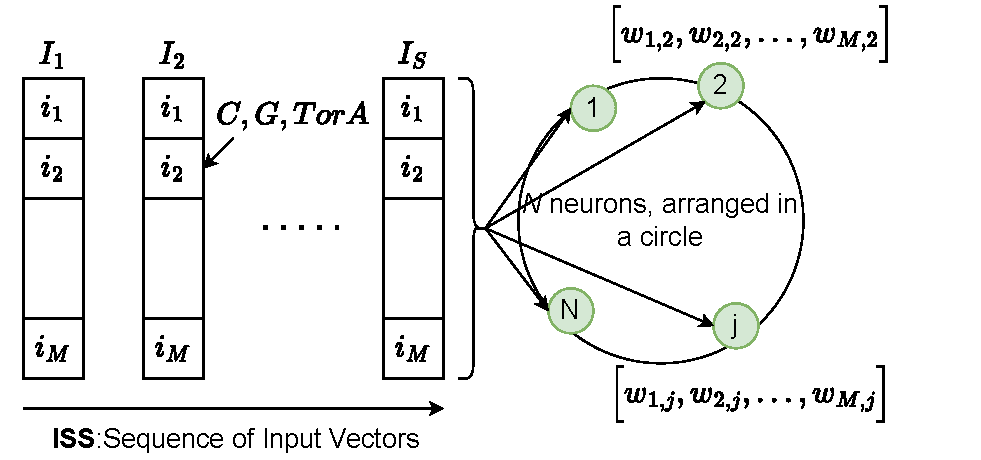
\includegraphics[width=0.6\textwidth]{SOMCircular.pdf}}
	\caption{SOM based Genomic Identification}
	\label{fig:algorithm}
\end{figure}

The training phase is for a specific bacterial genome. The objective of training a SOM network is to embed genomic features of a specific bacteria into a SOM. Each SOM network can be trained to recognize only one bacteria. In order to recognize a range of bacteria, many SOM networks need to be trained. During inference, when DNA sequences of unknown bacteria are compared with trained SOM networks, the SOM network trained with the same bacteria as the unknown test bacteria must have the highest correlation. Based on the correlation, we can identify the unknown bacteria. 

\algref{alg:algorithm} describes the actual training and inference processes. During the training process, the algorithm first tries to find the neuron with a minimum distance from the particular input vector. This neuron is considered a winning neuron. Then, the weights of the neighborhood of the winning neuron are updated based on the distance from the winning neuron. The training process is repeated for all training vectors, and the SOM learns the features of that particular bacterial genome.

Random weights initialize the weight matrix. The complete bacterial DNA sequence is chopped randomly into a set of fixed-size training sequences, the $IS$ in \algref{alg:algorithm}, line~\ref{IS_Def}. On the line~\ref{beta_init}, parameters $\beta_{min}$, $decay\_factor$, and $\beta$ are initialized. $\beta$ is used to control the converging process of SOM. $\beta$ is decreased by the factor $decay\_factor$ at each step of the converging process, and $\beta_{min}$ is the minimum value $beta$ can attain. In line~\ref{dist_min} and~\ref{j_min}, the training process first tries finding the winning neuron. Then, weights of the neighborhood of the winning neuron are updated based on the distance between the target neuron and the winning neuron, as shown in line~\ref{dist_update} and~\ref{W_update}. Finally in line~\ref{beta_update}, the parameter $\beta$ is decreased by $decay\_factor$. After repeating the training process for all training vectors in the input sequence $IS$, the SOM would have learned the features of that particular bacterial genome. 

During the inference phase, some test DNA fragments from one unknown bacteria are sent to each trained SOM network. The SOM network that correlates the test input sequence best is chosen as the winning SOM, and the bacteria it represents reveals the identity of the unknown test bacteria. The correlation measurement is marked by the score shown in \algref{alg:algorithm} line~\ref{score}. The smaller the score is, the better it correlates with the input test vectors.
\begin{algorithm}[htb]
	 \caption{Pseudo code SOM learning and inference for genome identification}
	\label{alg:algorithm}
	\begin{algorithmic}[1]\label{Algo:SOMTraining}
%		\Procedure{SOMTraining}{$N,I,IS,W$}
		\Statex \mbox{\textbf{Algorithm Part 1}: SOM training for 1 bacterial genome}
		\State \textbf{Input} $N:$ Number of neurons
		\State \textbf{Input} $I{=}[i_1, i_2, ..., i_M]$: Input-Vector
       	\State \textbf{Input} $IS{=}{I_1, I_2, ..., I_S}$: Sequence of Input-Vectors, each IS represents one bacterial genome \label{IS_Def}
       	\State \textbf{Input} $W_{i,j}: M\times N$ weight matrix for 1 bacteria
        \State $\beta_{min}=0.01$; $decay\_factor=0.99$; $\beta=1.0$\label{beta_init}
		\For{$I_k \in IS$}
		\State $dist_{min}=\min\limits_{j=1...N}(\sum_{i=1}^{M}|I_{k,i}-W_{i,j}|)$\label{dist_min}
        \State $j_{min} = j$ where $dist_{j} = dist_{min}$\label{j_min}
        \For{$j \in 1...N$}
           \State $dist = \frac{N}{2} - ||j-j_{min}|-\frac{N}{2}|$\label{dist_update} \Comment{toroid distance}
           \State $W_j = W_j - \frac{\beta}{2^{dist}}(W_j-I_k)$\label{W_update}
        \EndFor
        \State $\beta = \min(\beta*decay\_factor, \beta_{min})$\label{beta_update}\Comment{decay $\beta$}
		\EndFor
%		\EndProcedure
%    \Procedure{SOMInference}{$N,I,IS,W$}
  \Statex
   \mbox{\textbf{Algoritm Part 2}: SOM inference}
    \State \textbf{Input} $TIS{=}{I_1, I_2, ..., I_S}$: Test Input Sequence of Input-Vectors for which the bacteria is to be identified
    \State \textbf{Input} $W_{r,j,i}{=}R\times N \times M$: Weights for R bacteria
    \State $Inferred\_r$ is $r$ with\label{inferred_r}
    \State $score{=}\min\limits_{r=1...R}\Bigl[\sum_{k=1}^{S}\min\limits_{j=1...N}(\sum_{i=1}^{M} |I_{k,j}-W_{r,i,j}|)\Bigr]$\label{score}
%   \EndProcedure		
	\end{algorithmic}
\end{algorithm}
\section{Low bit-width FPGA Design of SOM}\label{custom}
In this section, we present the FPGA implementations that were used to implement SOM for the identification of bacterial genomes. The FPGA implementation is done on Xilinx Virtex7 485t chip to identify bacterial genomes. 

A custom semi-systolic array was hand-crafted for each of the different bit width implementations to analyze the area versus energy trade-off. The design takes a vector of weights as input and finds the neuron in the network closest to that input vector. This neuron is referred to as the winning neuron of the network. During the inference phase, the design outputs the distance between the input vector and the closest neuron's weights vector. This distance or score is used for identifying the bacteria in the test samples. During the training phase, neurons' weights are updated according to their distances from the winning neuron after finding the winning neuron.
\begin{figure}[h]
	\centering
	\captionsetup{font=sf}
	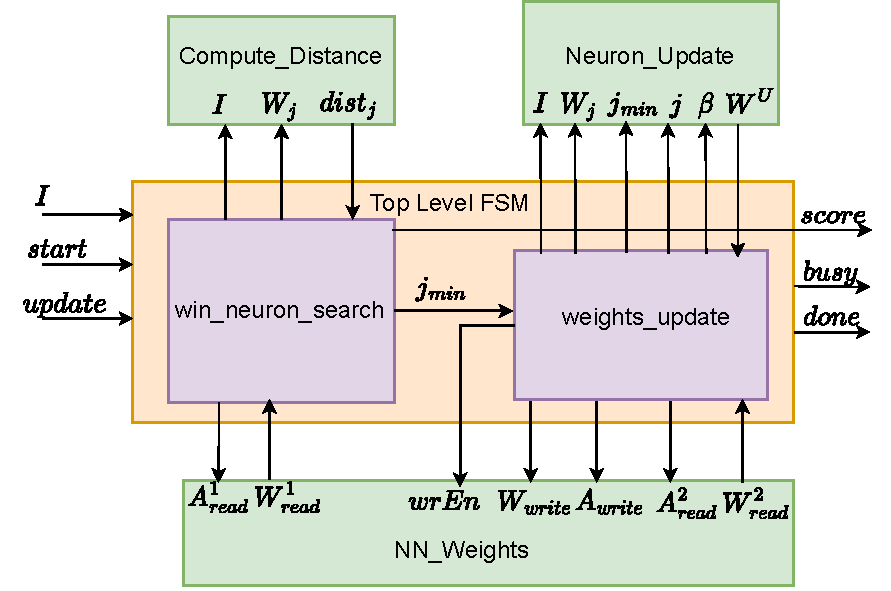
\includegraphics[width=0.7\columnwidth]{SomFpgaDesign}
	\caption{High level block diagram of the FPGA Implementation of BioSOM.}
	\label{fig:SOMFPGAImplementation}
\end{figure}
\begin{comment}

Figure \ref{fig:SOMFPGAImplementation} shows a high level block diagram of the FPGA implementation of BioSOM. The design takes inputs ($I{=}[I_1,I_2,...I_M]$) an input-vector of $M$ symbols, a $start$ and an $update$ signal. Each pair of bits in the input represents one of nucleotide A,C,G or T. Thus an input vector of $M$ symbols is represented by $2M$ bits word. Same FPGA design is used for inferencing and training the SOM network. $update$ signal is used to indicate if the inference or training of network needs to be performed. The design outputs the $busy$ signal, an integer $score$, and $done$ signal. $busy$ signal is output as 0 if the design is ready to accept the next input-vector else set to 1. The $score$ value is the distance of the input-vector from the wining neuron. The $score$ is valid when the $done$ singal is set to 1. 

The key components of the design are Compute\_Distance, Neuron\_Update, and NN\_Weights.
NN\_Weights reads and updates the NN weights in BRAM, Compute\_Distance computes the distance of the input-vector ($I$) from a single neuron, and Neuron\_Update computes the updated weight vector of a neuron.
The top level FSM iterates all the neurons of the SOM, reads the neuron weights using NN\_Weights. It then computes the distance of the neurons ($dist_j$) from $I$ using Compute\_Distance and updates ($dist_{min}$) and index of the winning neuron ($j_{min}$). During the inference phase ($update{=}0$), after computing the distance from all the neurons, the top level FSM returns $dist_{min}$ as a $score$ to determine the matching bacterial genome and sets the $done$ signal to 1. 

Training phase ($update{=}1$), after finding the wininng neuron index ($j_{min}$), involves additional step for computing and updating the weight vectors of neurons. The top level FSM iteratively reads the neurons weights vector using NN\_Weights and invokes Neuron\_Update and passes the neuron weights vector ($W$), input vector ($I$), the wining neuron index ($j_{min}$), and network parameters $\beta$ as inputs. Neuron\_Update returns the updated neuron weights vector ($W^U$) which is stored in BRAM by top level FSM using the NN\_Weights. 

The Neural Network weights are stored in 2-dimensional array in BRAMs. $1^{st}$ dimension represent neurons in the network and $2^{nd}$ dimension holds the weights of each neuron. Let us assume there are N neurons in the network, each neuron has M weights, and each weight is stored as a fixed-point number. Bit width analysis is performed by varying the number of bits (8, 12, 16, 24 and 32) used to represent the weights. The design is configurable for $N$, $M$ and number of bits to represent each weight. 
\end{comment}
\figref{fig:SOMFPGAImplementation} presents a high-level block diagram of the FPGA implementation of BioSOM. The design takes input as an input vector ($I = [I_1, I_2, ..., I_M]$), where $M$ symbols are represented by pairs of bits corresponding to nucleotides A, C, G, or T. Therefore, the input vector of $M$ symbols is represented by a word of $2M$ bits. The FPGA design serves to infer and train the SOM network, using a $start$ signal to initiate the process and an $update$ signal to distinguish between inference and training operations. The design outputs three signals: $busy$, $score$, and $done$.
$busy$ signal is set to 0 when the design is ready to accept the next input vector and 1 when busy processing the current input. $score$ represents the distance of the input vector from the winning neuron as an integer value. The $score$ value is valid after the $done$ signal is set to 1. $done$ signal indicates the completion of the distance computation. The key components of the design are as follows:
\begin{itemize}
	\item Compute\_Distance: This module calculates the distance between the input-vector ($I$) and a single neuron.
	\item Neuron\_Update: This module computes the updated weight vector of a neuron during the training phase.
	\item NN\_Weights: This module reads and updates the Neural Network (NN) weights stored in Block RAM (BRAM).
\end{itemize}
The top-level FSM (Finite State Machine) iterates through all the neurons in the SOM. For each neuron, it reads the neuron's weights using NN\_Weights, computes the distance of the neuron from the input-vector ($I$) using Compute\_Distance, and updates the minimum distance ($dist_{min}$) and the index of the winning neuron ($j_{min}$). During the inference phase ($update{=}0$), the FSM returns $dist_{min}$ as the $score$, determining the matching bacterial genome, and sets the $done$ signal to 1.

During the training phase ($update{=}1$), after identifying the winning neuron index ($j_{min}$), additional steps are performed to compute and update the weight vectors of neurons. The top-level FSM iteratively reads the neurons' weight vectors using NN\_Weights and invokes Neuron\_Update. It passes the neuron weights vector ($W$), input vector ($I$), the winning neuron index ($j_{min}$), and network parameter $\beta$ as inputs. Neuron\_Update returns the updated neuron weights vector ($W^U$), which is then stored in BRAM by the top-level FSM using NN\_Weights.

The Neural Network weights are stored in a 2-dimensional array in BRAMs, where the first dimension represents the neurons in the network, and the second dimension holds the weights of each neuron. Assuming there are N neurons in the network, each neuron has M weights, and each weight is stored as a fixed-point number. The bit-width analysis is performed by varying the number of bits (8, 12, 16, 24, and 32) used to represent the weights. The design is configurable for $N$, $M$, and the number of bits used to represent each weight.
\begin{figure}[!htb]
	\centering
	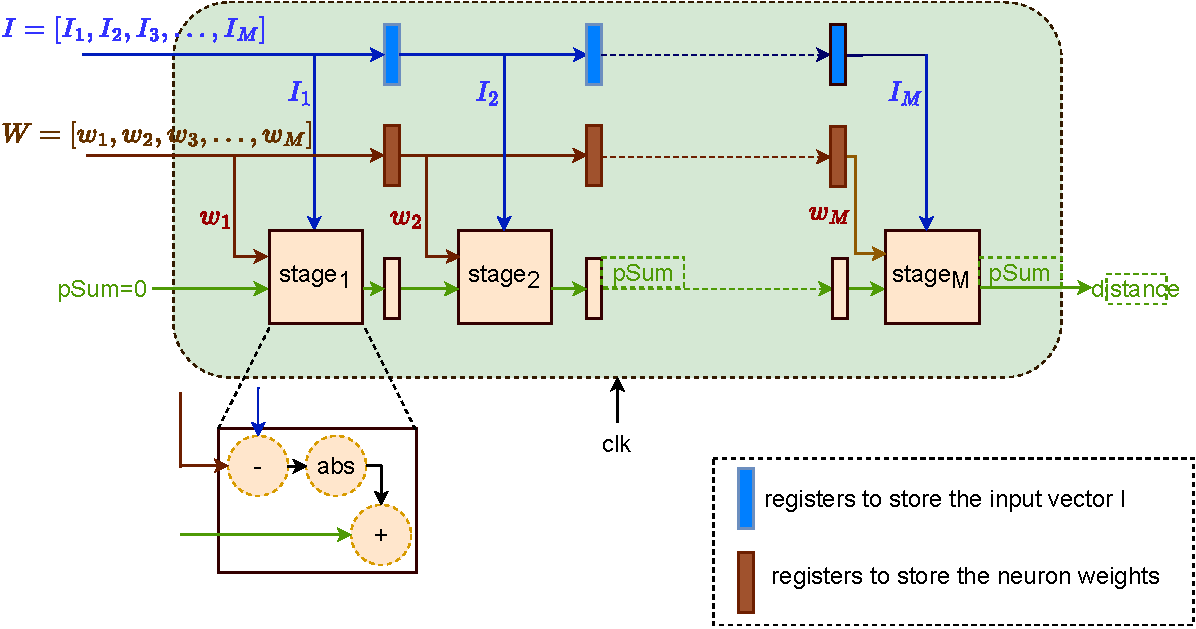
\includegraphics[width=0.7\columnwidth]{computeDistance}
	\caption{Pipelined implementation of Compute\_Distance with M stages and Initiation Interval (II)=1 .}
	\label{fig:ComputeDistance}
\end{figure}
\begin{comment}
\figurename{~\ref{fig:ComputeDistance}} shows the design of the Compute\_Distance module. This component takes an input-vector ($I$) and a neuron weight vector ($W$) as input and returns the distance between neuron weights and the input vector ($\sum_{i=1}^{M}|I_{i}-W_{i}|$) as described in Algorithm~\ref{alg:algorithm}. This component has a pipelined implementation with $M$ number of pipeline stages. The initiation Interval (II) of this component is 1. Each stage of the pipeline computes the absolute difference between one input element and the corresponding neuron weight and accumlates the difference into the partial sum (pSum) as shown in \figurename{~\ref{fig:ComputeDistance}}. The accumlated pSum is then passed as input to the next stage. The pSum to the first stage is set to zero. The pSum of the last stage is the distance between the input and neuron vectors.
\end{comment}

\figurename{~\ref{fig:ComputeDistance}} illustrates the design of the Compute\_Distance module. This module takes an input-vector ($I$) and a neuron weight vector ($W$) as inputs and computes the distance between the neuron weights and the input vector ($\sum_{i=1}^{M}|I_{i}-W_{i}|$) using the algorithm described in \algref{alg:algorithm}. 

The Compute\_Distance module is implemented with pipelining, and it consists of $M$ pipeline stages. The Initiation Interval (II) of this component is 1, meaning that each stage of the pipeline can be initiated in consecutive clock cycles. Each pipeline stage computes the absolute difference between one element of the input vector and the corresponding neuron weight and accumulates the difference into a partial sum (pSum), as shown in \figurename{~\ref{fig:ComputeDistance}}.

To elaborate, the pSum accumulated in one stage is passed as input to the next stage, creating a data flow through the pipeline. The pSum for the first stage is initialized to zero, and at the last stage, the pSum represents the distance between the input and neuron vectors.

The \textit{Neuron Update} has seven stages pipelined design with II=1. The pipeline stages are shown in Figure \ref{fig:NeuronUpdate}. Neuron\_Update takes inputs the weights vector ($W$), index of the neuron ($j$), the input vector ($I$), the wining neuron index ($j_{min}$), and the $\beta$ and outputs the updated weights vector $W_U$. 
It first computes the distance ($dist$) of the input neuron from the winning neuron (Algorithm~\ref{alg:algorithm}, line~\ref{dist_update}) and then computes the update factor ($\frac{\beta}{2^{dist}}$). Neuron\_Update then updates the weights using the update factor (Algorithm~\ref{alg:algorithm}, line~\ref{W_update}). 
\begin{figure}[!htb]
	\centering
	\includegraphics[width=0.7\columnwidth]{neuronUpdate}
	\caption{Pipelined Implementation of Neuron\_Update with 7 stages and Initiation Interval (II)=1.}
	\label{fig:NeuronUpdate}
\end{figure}

If $N$ is the number of neurons in the SOM network and each neuron has $M$ weights, determining the winning neuron takes $M{+}N$ cycles. The latency of the inference phase is $M$ and $II{=}1$. The weight update for an input vector can only start after the top-level FSM determines the winning neuron index ($j_{min}$). After finding the winning neuron, Neuron\_Update takes seven cycles to update the weight vector of the first neuron and then $N{-}1$ cycles to update the weights of the remaining $N{-}1$ neurons. For a given input vector, these two components can execute sequentially. However, while Neuron\_Update is processing $i^{th}$ input vector, Compute\_Distance can start its operations for the next $(i{+}1)^{th}$ input vector immediately after the first weight is updated by Neuron\_Update at $((M{+}N){+}7)^{th}$ cycle for the $i^{th}$ input vector. In this way Compute\_Distance and Neuron\_Update components can overlap their execution, processing different input vectors at the same time. This design has overall $II{=}M{+}N{+}7$ cycles for the training phase.

\section{Experimental Results And Analysis}\label{sec:results}
In this section, we present the results of our experiments. In subsection \ref{ex_setup}, we give the details of our experimental setup used for measuring the accuracy of the SOM. Subsections \ref{fpga_results} describe the experimental setup and present the results of the FPGA implementation.
\subsection{Accuracy experimental setup}\label{ex_setup}
The SOM has been implemented with a range of fixed-point formats. With fewer bits, one naturally expects the SOM network for bacterial identification to suffer from accuracy degradation. A MATLAB simulation model was created to analyze the accuracy loss using fixed-point implementation. The experiment used a scaled-down version of the bacterial identification problem to reduce the training time of the network. We consider that this does not compromise the resulting accuracy of the SOM. We trained 10 SOMs with ten different bacteria DNA sequences. Each SOM network has 100 neurons inside, and each neuron has 20 weights. We trained the networks with two independent training processes running in parallel. One is implemented using double precision floating point, and the other is implemented with fixed-point weights. After training, we used the trained networks to identify the unknown sequence and record their scores.

Two metrics are defined to evaluate the implementation accuracy. The \emph{quantization error} is defined as the relative error between fixed-point format score ($S_{fixed}$) and double-precision floating-point format score ($S_{float}$):
\begin{align*}
	quantization\_error = \frac{|S_{fixed} - S_{float}|}{S_{float}}\times 100\%
\end{align*}
Assuming the double precision floating format has no classification error, the \emph{classification error} for the fixed-point format is defined as the ratio of the number of times the network classified ($C_{false}$) the bacterial strain to the total number of tests performed ($C_{total}$):
\begin{align*}
	classification\_error = \frac{C_{false}}{C_{total}}\times 100\%
\end{align*}
Classification and quantization errors are not entirely independent but reveal the different aspects of fixed-point implementation accuracy. Quantization error shows the difference between fixed-point representation and golden double-point reference. It does not change with the problem. Classification error determines the final impact of the accuracy loss introduced by the fixed-point implementation and is problem dependent. Figure \ref{fig:error} presents the quantization and classification errors depending on the bit resolution. From the figure, 8-bit representation completely fails the experiment, 12-bit has 39\% classification error, 16-bit has $<$1\%, and 24-bit and 32-bit successfully pass the experiment with 0\% of classification error. However, we should notice that though 16-bit pass the test, it still has about 10\% quantization error.\par
\begin{figure}[ht]
	\centering
	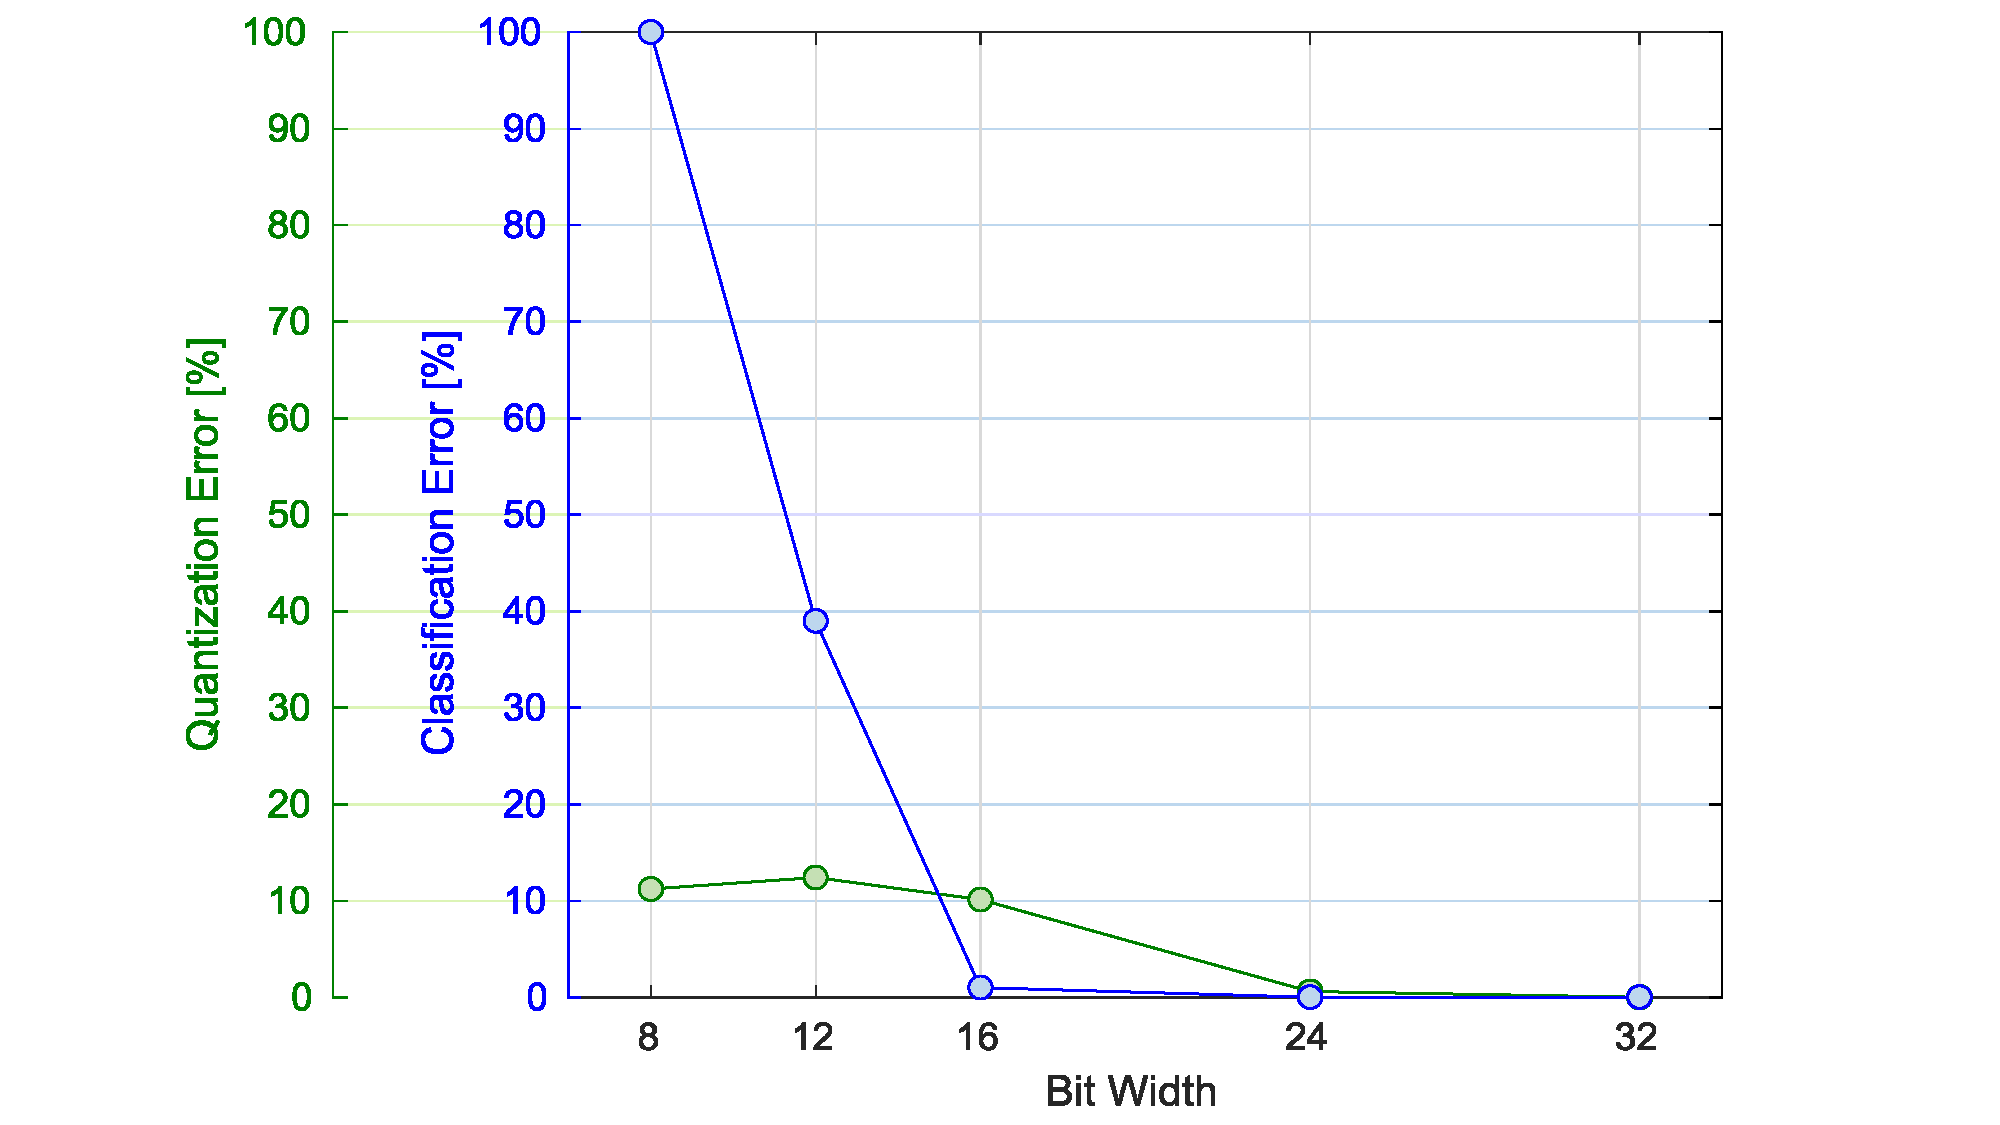
\includegraphics[trim=  85 5 130 8, clip, width=0.45\columnwidth]{accuracy}
	\caption{Quantization error compared to the identification error.}
	\label{fig:error}
\end{figure}
Each SOM was trained with a specific fixed-point resolution. The quantization error shows the difference of the \emph{score} variable, see algorithm \algref{alg:algorithm}, between the fixed-point and the double precision. The quantization error is very important for the \emph{score} variable of the SOM, since this variable is the one that decides which is the winning SOM, i.e., which SOM matches the input DNA sequence. It is essential to guarantee sufficient bits for the \emph{score} of each SOM. If the resolution is too low, the \emph{score} of the SOMs after quantization will be identical even with low quantization error, making it impossible to identify the bacteria correctly. This explains that the quantization error is low in \figref{fig:error}, but the classification error is high in the 8 to 12-bit resolution region.
\subsection{FPGA experimental setup}\label{fpga_results}
This section presents the experimental results of the FPGA implementations presented in section \ref{custom}. The FPGA design is implemented with Vivado v.2016.4 used to synthesize and analyze the HDL Designs. Our design is implemented in VHDL and validated using the Vivado simulator. Experimentation is done for different fixed point representations of weights by modifying parameters in VHDL code. 

\begin{table}[h!]
	\centering
	\caption{Resource Comparison of different fixed point formats}
	\label{table:somFpgaRes}
	\begin{tabular}{ c |c | c| c |c | c } 
		\toprule
		Resource & 8b & 12b & 16b & 24b & 32b \\ 
		\midrule
		LUTs & 1823 & 2611 &3196 & 4375 & 5549 \\
		\hline
		Registers & 3481 & 4679 & 5871 & 8255 & 10639 \\ 
		\hline
		Slice & 854 & 1158 & 1369 &1809 & 2395 \\ 
		\hline
		LUT FF Pairs & 1007 & 1369 & 1750 & 2372 & 3043 \\
		\hline
		B-RAM & 4 & 6 & 8 & 11 & 15 \\
		\hline
		DSP48E1 & 17 & 17 & 17 & 17 & 33 \\
		\hline
		Bonded IOB & 57 & 61 & 65 & 73 & 81 \\
		\midrule
		%    \end{tabular}
	%\end{table}
	
	%\begin{table}[h!]
	%    \centering
	%    \caption{Power Comparison of different fixed-point formats}
	%    \label{table:2}
	%    \begin{tabular}[t]{ c |c | c| c |c | c } 
		\midrule
		Power(W) & 8b & 12b & 16b & 24b & 32b \\ 
		\midrule
		Total Power & 0.295 &0.314 &0.332 &0.356 &0.392 \\
		\hline
		Dynamic &0.052 &0.071 &0.089 &0.113 &0.148 \\ 
		\hline
		Device Static &0.243 &0.243 &0.243 &0.244 &0.244 \\ 
		\bottomrule
	\end{tabular}
\end{table}

The area and power numbers for different weight resolutions are extracted from the reports generated by the Vivado tool post placement and routing with a working frequency of 100 MHz.
\tabref{table:somFpgaRes} compares the resources and area for 8, 12, 16, 24, and 32 bits fixed point formats for a SOM network with 512 neurons. The second part of the table compares the average power in the different fixed point formats for the same SOM.

\begin{figure}[htb]
	\centering
	\subfloat[FPGA LUT utilization]{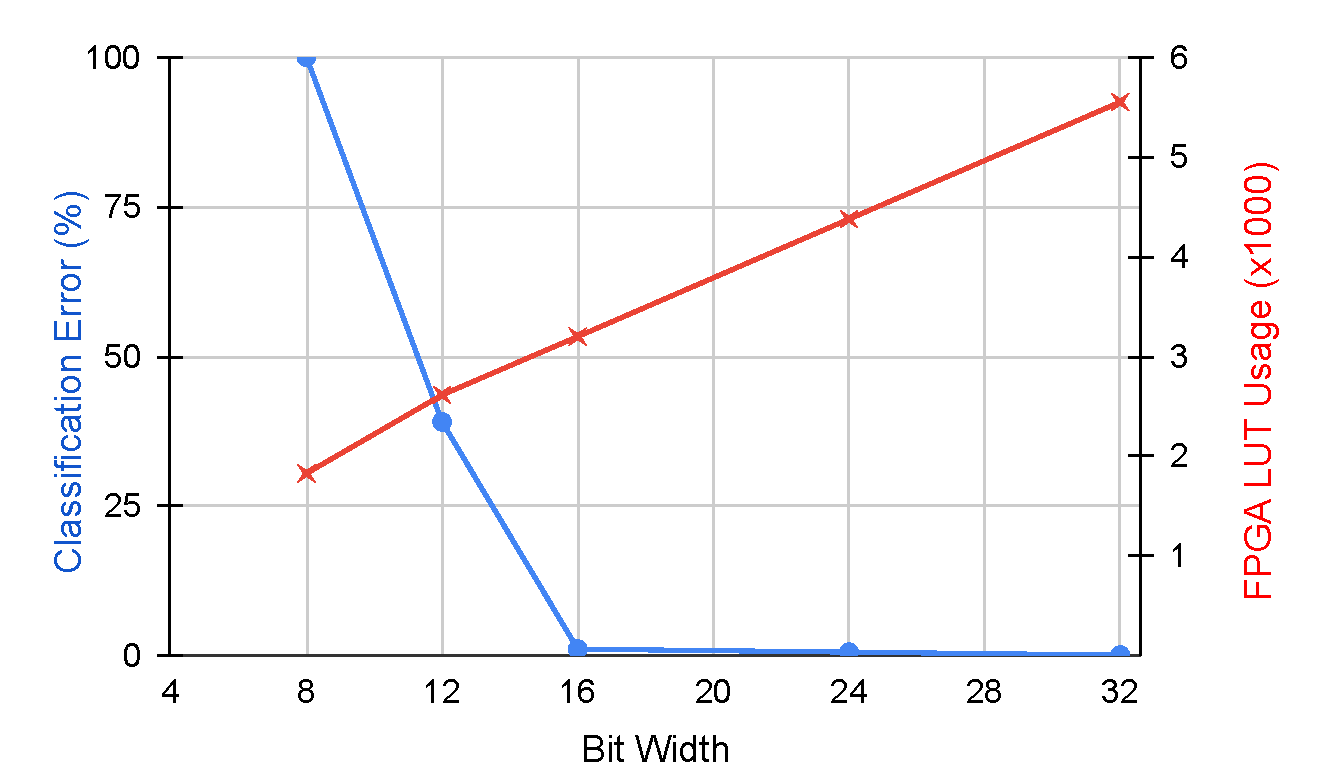
\includegraphics[width=0.45\columnwidth]{area}
		\label{fig:area}
	}~
	\subfloat[energy of FPGA implementation]{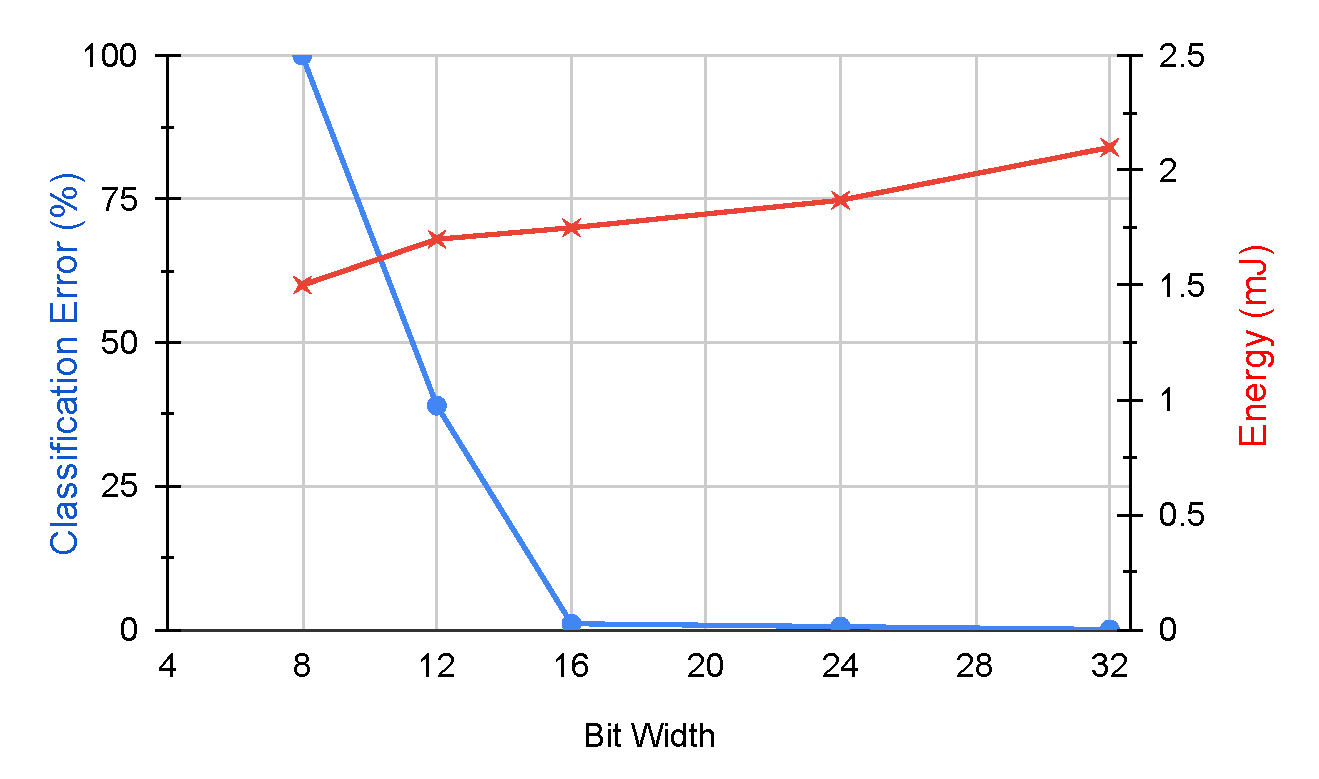
\includegraphics[width=0.46\columnwidth]{energy}
		\label{fig:energy}
	}
	\caption{ Area and energy comparison for different fixed-point format.}
	\label{fig:metrics}
\end{figure}
The results are summarized in \figref{fig:area} and \figref{fig:energy}. Both the amount of utilized LUTs and total energy in Joule is presented against the classification error. From the figures, we can easily conclude that we can substantially reduce the resources used and the energy by using a 16-bit fixed-point representation without losing accuracy. We can reduce the resources even further by moving to the 12-bit representation by sacrificing 39\% the SOM accuracy. 
\section{Summary}
\begin{comment}
In this work we explore the design space of a self-organizing map (SOM) used for rapid and accurate identification of bacterial genomes. This is an important health care problem.  The  SOM is trained on Next Generation Sequencing (NGS) data and is able to identify the exact strain of bacteria. This is in contrast to conventional methods that require genome assembly to identify the bacterial strain. In this work SOM has been implemented on FPGA. To lower the energy consumption, we exploit the robustness of SOM by successively lowering the resolution to gain further improvements in efficiency and lower the implementation cost without substantially sacrificing the accuracy. We do an in depth analysis of the reduction in resolution vs. loss in accuracy as the basis for designing a system with the lowest cost and acceptable accuracy using NGS data from  samples containing multiple bacteria from the labs of one of the co-authors. The objective of this method is to design a bacterial recognition system for battery operated clinical use where the area, power and performance are of critical importance. We demonstrate that with 39\% loss in accuracy in 12 bits and 1\% in 16 bit representation can yield significant savings in energy and area.

In this work, different bit width FPGA designs of SOM were implemented to enable trade-offs between accuracy and computation cost. Experiments has shown the big design space, resulting in different cost in terms of timing, area as well as energy, all of which are affected significantly by the fixed-point format representation. Through the experiment, we conclude that the SOM network with 16-bit fixed-point representation implemented on FPGA, has better benefits compared to other fixed-point formats with more bits. And 16-bit has acceptable classification error. Format with bits more than 16 no longer add any benefit to lower the classification error. 

In future works, we plan to apply more sophisticated methods to scale down the bit width without losing too much accuracy. For example, the weights can be dynamically scaled after several epochs of training when the current fixed point format is not suitable anymore. We are confident that, with such approximate computing techniques, we could possibly reduce the resolution to 8 bits with acceptable loss of accuracy and, by extension, the implementation cost of SOM networks on hardware.
\end{comment}
This chapter discusses using Self-Organizing Maps (SOM) for rapid genome identification, specifically for bacterial genomes. The chapter explores the benefits and limitations of using low bit-width resolution for representing weights in the SOM and its impact on accuracy, resource utilization, and energy efficiency in hardware implementations.

We present a design space exploration of SOM using different bit resolutions (8, 12, 16, 24, and 32 bits) for representing the neural network weights. We analyze the impact of these bit resolutions on the accuracy of SOM and their benefits for hardware implementation. The trade-off between accuracy and hardware efficiency is explored by training multiple SOMs with different bit representations and comparing their performance.

The experimental setup includes a MATLAB simulation model to measure accuracy loss when using fixed-point implementations of the SOM. The quantization and classification errors are metrics to evaluate the accuracy of different bit resolutions. The results show that an 8-bit representation completely fails the experiment, while 12-bit has a high classification error but a lower quantization error. 16-bit representation exhibits minimal classification error but still has a quantization error of around 10\%. On the other hand, 24-bit and 32-bit representations successfully pass the experiment with 0\% classification error.

The FPGA implementation of SOM is presented, aiming at bacterial genome identification. The design is configurable for different numbers of neurons, weight dimensions, and bit resolutions. We utilize pipelining and parallelization techniques to optimize the hardware design for efficiency. Resource utilization and power consumption are compared for different bit representations.

The experimental results show that a 16-bit fixed-point representation provides a good balance between resource utilization, energy efficiency, and accuracy. It significantly reduces resources compared to higher-bit representations (24 and 32 bits) while maintaining almost the same accuracy. A 12-bit representation further reduces resource usage but sacrifices accuracy.

In conclusion, the chapter highlights the benefits of using low bit-width resolution in the hardware implementation of SOM for genome identification. A 16-bit representation is found to be a practical choice, offering significant savings in resources and energy consumption without compromising accuracy. The study provides valuable insights into the trade-offs in optimizing SOM for efficient hardware implementations in genome recognition applications.